% *******************************************************************************
% * Copyright (c) 2007 by Elexis
% * All rights reserved. This document and the accompanying materials
% * are made available under the terms of the Eclipse Public License v1.0
% * which accompanies this distribution, and is available at
% * http://www.eclipse.org/legal/epl-v10.html
% *
% * Contributors:
% *    G. Weirich - initial implementation
% *
% *  $Id: customize.tex 2930 2007-07-28 16:43:29Z rgw_ch $
% *******************************************************************************
% !Mode:: "TeX:UTF-8" (encoding info for WinEdt)

\section{Funktionsprinzip}
Hervorstechendstes Merkmal vom Elexis ist die grosse Flexibilität. Wenn Sie ein anderes Praxisprogramm gewöhnt sind,
wird Ihnen die Bedienung von Elexis vielleicht etwas ungewöhnlich vorkommen. Wir möchten deshalb hier zunächst einige
grundsätzliche Konzepte erläutern.
\index{Bedienungskonzepte}
 \subsection{Schreibtisch / Perspektive}
Stellen Sie sich Ihren Arbeitstisch vor. Vermutlich werden Sie sich im Lauf der Zeit angewöhnt haben,
bestimmte Dinge an einen bestimmten Ort auf Ihrem Schreibtisch zu legen, also
Arbeitsfunktionen einem Ort zuzuordnen, wo sie sie jeweils
(idealerweise) leicht wiederfinden. Ihre Anordnung ist nicht unbedingt dieselbe wie bei jemand anderem,
der dasselbe Schreibtischmodell besitzt.

Das Programmfenster von Elexis ist so ein Schreibtisch (s. fig. \ref{fig:tour1}.Es ist in
keiner Weise festgelegt, welche Funktion
wo zu finden ist, ja es ist nicht einmal festgelegt, welche Elemente überhaupt
auf dem Schreibtisch erscheinen, und welche vielleicht irgendwo
in einer Schublade verstaut sind und nur bei Bedarf hervorgeholt werden müssen.

%\usepackage{graphics} is needed for \includegraphics
\begin{figure}[htp]
\begin{center}
  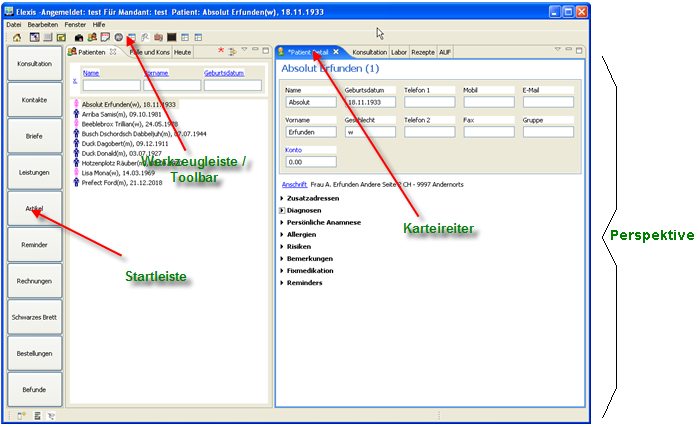
\includegraphics[width=0.9\textwidth]{images/tour1}
  \caption{Standard-Perspektive}
  \label{fig:tour1}
\end{center}
\end{figure}

Eine Anordnung von Arbeitsflächen nennen wir eine 'Perspektive' (Perspective). Die einzelnen Funktionseinheiten
(oben 'Patienten' und 'Patienten-Detail'), aus denen sich die Perspektive zusammensetzt bezeichnet
man als 'Ansicht' (View).

\subsubsection{Perspektive und Views}

Oben (fig. \ref{fig:tour1} sehen sie als Beispiel eine Perspektive, die für
einen kleinen Bildschirm geeignet ist, es zeigt einen
Screenshot auf einem 15-Zoll-TFT-Monitor. Die Ansichten \glqq
Patienten\grqq{}(links) und \glqq Patient Detail\grqq{}(rechts) liegen obenauf,
andere Ansichten sind dahinter angeordnet, so dass nur ein Karteireiter oben
zu sehen ist.
Auf einem grösseren Bildschirm würden Sie vermutlich eine andere Anordnung
bevorzugen: fig. \ref{fig:tour2} zeigt einen Screenshot auf einem
17-Zoll-TFT-Monitor mit mehreren Views gleichzeitig.

%\usepackage{graphics} is needed for \includegraphics
\begin{figure}[htp]
\begin{center}
  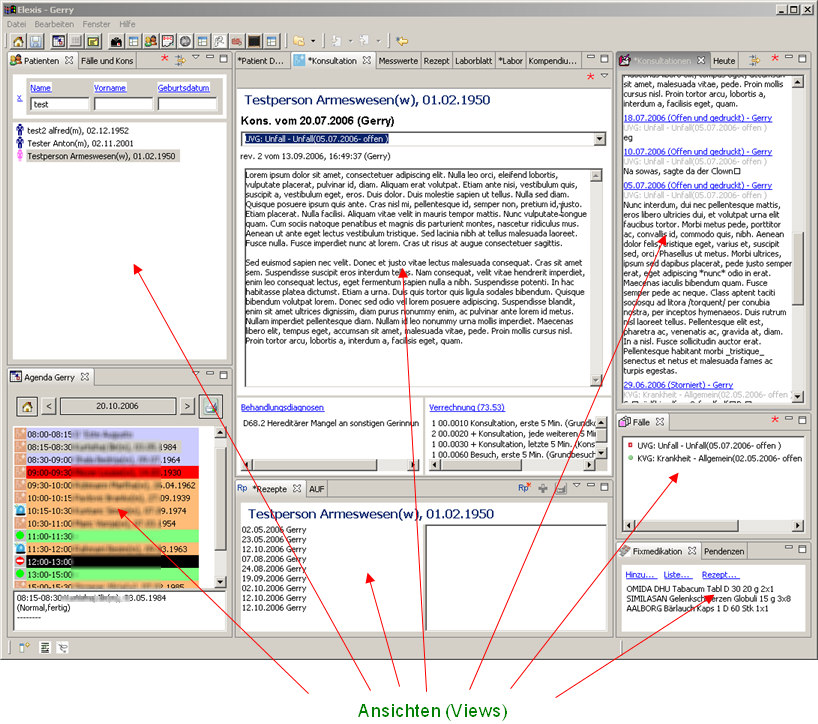
\includegraphics[width=0.9\textwidth]{images/tour2}
  \caption{Komplexere Perspektive}
  \label{fig:tour2}
\end{center}
\end{figure}
\textbf{Ansichten}

\subsubsection{Ansichten / Views}
Jede Ansicht entspricht einer bestimmten Funktionalität. Im abgebildeten Fenster sehen sie die Ansicht einer
Patientenliste (links) und die Details des 'aktiven' Patienten (rechts). Es gibt weitere Ansichten wie KG-Eintrag des aktuellen Patienten, eine Liste aller KG-Einträge, die Fixmedikation, die Rezepte,die Arbeitsunfähigkeitszeugnisse,
die Agenda etc. Jede Ansicht ist eine definierte \glqq Sicht\grqq auf die vorhandenen Daten,
daher der Name \glqq Ansicht\grqq. Sie lassen sich über die Reiter aktivieren. Die
Reiter selber lassen sich beliebig anordnen, aktivieren oder deaktivieren.

Egal wie Sie die Views angeordnet haben, jede View lässt sich zur besseren
Übersicht jederzeit auf Vollbildgrösse bringen, indem man auf den Reiter
doppelklickt (s. Abb. \ref{fig:tour3}).

\begin{figure}[htp]
\begin{center}
  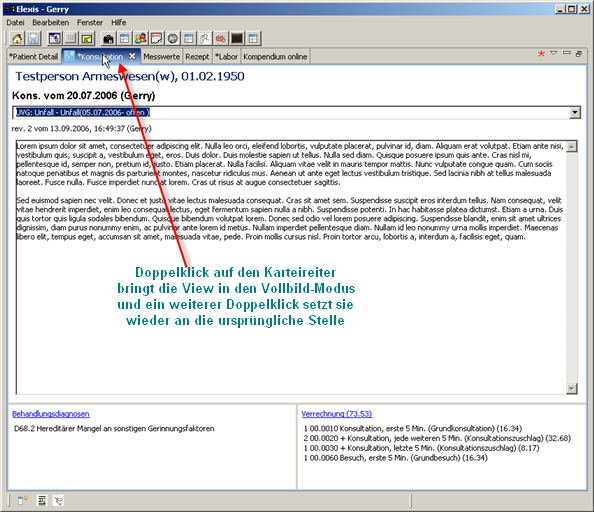
\includegraphics[width=0.9\textwidth]{images/tour3}
  \caption{View maximieren}
  \label{fig:tour3}
\end{center}
\end{figure}

\subsubsection{Views und Perspektiven anpassen}


In der Standard-Startperspektive ist links eine \glqq Startleiste\grqq{} zu
sehen. Diese führt Sie zu vordefinierten Perspektiven - es erscheinen in diesen
jeweils die passenden Ansichten. Die Werkzeugleiste führt, wie bei anderen
Programmen üblich, zu verschiedenen Funktionen. Jede Ansicht hat einen
Karteireiter, über den sie in den Vordergrund gebracht oder maximiert werden kann.

Sie können die Fensterinhalte und Ansichten völlig frei gestalten.


Die Programmfenster-Inhalte lassen sich jederzeit anpassen:
\begin{itemize}
  \item Sie können nicht benötigte Ansichten entfernen damit sie mehr Platz für
  die verbleibenden Ansichten haben
	\item können Views in der Horizontalen und Vertikalen vergrössern oder verkleinern
	\item können Views an beliebige andere Stellen des Bildschirms schieben (indem Sie sie
	an den Reitern mit gedrückter linker Maustaste \glqq festhalten\grqq{})
\end{itemize}

Jede Zusammenstellung kann als Perspektive gespeichert werden - und ist als
solche auf einfache Art wieder aufrufbar.

\subsection{Perspektiven einrichten und speichern}
Sie können nicht nur eine Perspektive erstellen, sondern beliebig viele. Ihre MPA braucht möglicherweise eine
andere Perspektive als Sie selber, z.B. wünscht sie sich die Agenda gross. Oder Sie selber verwenden unterschiedliche
Perspektiven, z.B. eine für Konsultationen und eine andere für die Buchhaltung oder wenn
Sie einen Bericht schreiben. Perspektiven lassen sich mit Elexis in wenigen Schritten zusammenstellen:\\

\bigskip

\textbf{Schritt 1: Benötigte Ansicht(en) öffnen}\\

Wählen Sie im Menu \textsc{Fenster - Ansicht - Andere}. Es öffnet sich ein Dialog wie in Abb. \ref{fig:cust1}.\\

\begin{figure}[htbp]
     \begin{minipage}{0.4\textwidth}
      \centering
       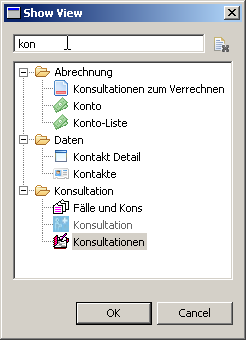
\includegraphics[width=0.8\textwidth]{images/customize1}
       \caption{View suchen}
       	\label{fig:cust1}
     \end{minipage}\hfill
     \begin{minipage}{0.5\textwidth}
        Diese Dialogbox zeigt Ihnen sämtliche Views, die in Ihrer Elexis-Installation vorhanden sind (Welche und wieviele das sind, hängt von den installierten Plugins ab). Wenn Sie in der obersten Zeile den Anfang der gesuchten View zu tippen beginnen, wird die Liste automatisch gefiltert.\\

     \end{minipage}

   \end{figure}

 \bigskip

\textbf{Schritt 2: Die Ansichten an die gewünschte Stelle schieben und auf die gewünschte Grösse bringen}

   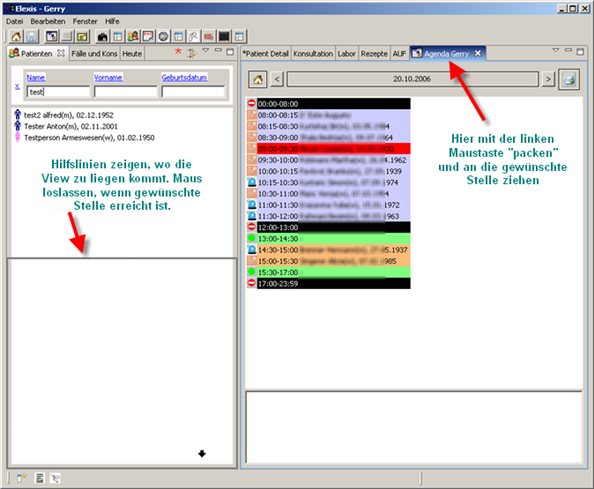
\includegraphics[width=0.8\textwidth]{images/agendagewaehlt}\\
   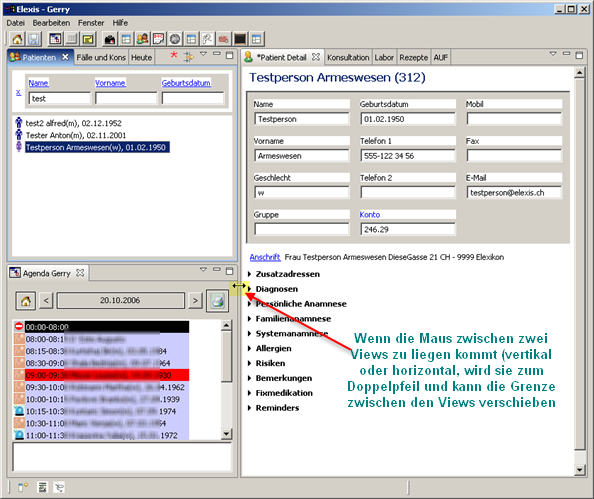
\includegraphics[width=0.8\textwidth]{images/agendaanpassen}

\bigskip
\textbf{Schritt 3:Perspektive speichern}\\
Wenn Sie möchten, dass Ihre so erstellte Perspektive auch bei späteren Programmstarts oder auf anderen Computern zur Verfügung steht, haben Sie mehrere Möglichkeiten:
\begin{itemize}
\item Wählen Sie im Menu \textsc{Fenster - Perspektive - als Startperspektive speichern}. Damit legen Sie fest, dass die eben zusammengestellte Perspektive fortan beim Anmelden erscheint.
\item \textsc{Fenster - Perspektive - speichern als...}. Damit können Sie die aktuelle Perspektive unter einem frei wählbaren Namen abspeichern. Sie können sie zu einem späteren Zeitpunkt jederzeit mit \textsc{Fenster - Perspektive - andere...} mit diesem Namen wieder zurückholen.
\item \textsc{Fenster - Perspektive - speichern}. In diesem Fall wird die aktuelle Perspektive unter ihrem bestehenden namen gespeichert.
\item Und, last but not least, Wenn Sie unter \textsc{Datei - Einstellungen - Anwender} die Perspektive unter einem bestimmten Namen speichern, dann können Sie sie auch von einer anderen Arbeitsstation aus unter diesem Namen einlesen\footnote{Dies geht allerdings natürlich nur, wenn auch auf der aufrufenden Arbeitsstation alle Views, die in dieser Perspektive definiert sind, auch vorhanden sind}. Diese Option eignet sich, um einheitliche Arbeitsumgebungen zuammenzustellen.
\end{itemize}

